\chapter{Running the Game: Core Procedures}
\label{ch:gm-core}
\index{GM procedures}\index{GM mindset}

% =========================================================
% CHAPTER QUICK-START BOX
% =========================================================
\begin{tcolorbox}[
  title={\textbf{Running Fate's Edge --- Core Procedures in Brief}},
  colback=blue!5!white,
  colframe=blue!75!black,
  boxrule=0.8pt,
  arc=3mm,
  fonttitle=\bfseries\large,
  left=8pt,
  right=8pt,
  top=8pt,
  bottom=8pt,
  sharp corners=southwest, % optional: smoother look
  enhanced
]

\small
\setlength{\parskip}{0.6\baselineskip}  % add space between paragraphs
\setlength{\parindent}{0pt}

\textbf{Your Job:} Frame pressure, track consequences, let the fiction move forward.

\medskip
\textbf{Default Settings} \quad DV = 3 \quad · \quad Position = Controlled \quad · \quad One short Clock

\medskip
\textbf{The Core Loop (every meaningful action)}
\begin{enumerate}[leftmargin=*, nosep]  % nosep reduces vertical spacing
  \item Player declares intent \& approach (Attribute + Skill)
  \item You state Position \& set relevant Clocks
  \item Player rolls d10s; count \textbf{Successes (6+)} \& \textbf{Story Beats (1s)}
  \item Compare to DV → use \textbf{Outcome Matrix}
  \item Apply consequences \& update the fiction
\end{enumerate}

\medskip
\textbf{Outcome Matrix (what you do)}
\begin{itemize}[leftmargin=*, nosep]
  \item \textbf{Clean Success} (S $\geq$ DV, SB=0) → intent achieved, no complication
  \item \textbf{Success with SB} (S $\geq$ DV, SB>0) → intent achieved, spend SB for a twist
  \item \textbf{Partial} (0 < S < DV) → progress made, player gains 1 Boon
  \item \textbf{Miss} (S = 0) → no progress, player gains 2 Boons, spend SB to escalate
\end{itemize}

\medskip
\textbf{Story Beats (SB) -- spend them to create drama}
\begin{itemize}[leftmargin=*, nosep]
  \item \textbf{1 SB:} Minor -- noise, tick a clock, small setback
  \item \textbf{2 SB:} Moderate -- alarm raised, lose advantage, worsen Position
  \item \textbf{3+ SB:} Major -- reinforcements, scene shift, break an asset
\end{itemize}

\medskip
\textbf{Golden Rule}\par
\emph{When in doubt, make a ruling that keeps the story moving.} \\
Set DV=3, Position=Controlled, ask for the roll, and resolve with the Outcome Matrix.

\end{tcolorbox}

\begin{effectbox}
  \textbf{Position} (Dominant/Controlled/Desperate) = How risky is this action? – determines severity of failure and re-rolls.\\
  \textbf{Effect} (Limited/Standard/Great) = How much do you achieve on a success? – determines scope, scale, or quality.
  
  \vspace{4pt}
  \small
  \textit{Example:} Disarming a trap – Limited Effect lets one person cross, Standard lets two, Great lets all four.
  \end{effectbox}

% =========================================================
% SELLING THE ACTION BOX (FIXED: No \subsection inside)
% =========================================================
\begin{tcolorbox}[
  colback=red!5!white,
  colframe=red!75!black,
  title=\textbf{Selling the Action -- When Players Give You Gold},
  fonttitle=\bfseries\large,
  sharp corners,
  drop shadow,
  before skip=10pt,
  after skip=10pt
]

\textit{"Don't just tell me you swing your sword. Show me the dust in your eyes, the tremble in your arm, the desperate prayer you whisper to the Traveler."}
\textit{"And don't just paint a pretty picture -- show me what your character risks, fears, or loves in this moment."}

\medskip
When a player \textbf{sells the action} -- not by piling on adjectives, but by revealing what their character cares about, what they stand to lose, or why this moment matters -- you have permission to give them a mechanical edge. This is a reward for \textbf{roleplay investment}, not vocabulary.

\medskip
\noindent\textbf{How to Rule It}
\begin{itemize}
  \item \textbf{Basic description:} "I attack the goblin." -- No bonus.

  \item \textbf{Tactical description:} The player uses the environment, positioning,
        or a clever tactic.  
        \textit{Example:} "I feint high, then drive my shoulder into the goblin's
        shield, shoving it aside to open its flank."  
        → \textbf{Improve Position by one step} (e.g., Controlled → Dominant)
        for this roll.

  \item \textbf{Character‑driven description:} The player states a stake, invokes
        a bond, reveals a fear, or makes a hard choice visible. \textit{One
        heartfelt sentence counts more than a paragraph of adjectives.}  
        \textit{Example:} "I think of my mother, who died because I wasn't brave
        enough. I won't let that happen again. I plant my feet and dare the
        goblin to come through me."  
        → \textbf{Improve Position by one step \textit{and} bank 1 Story Beat}
        (or upgrade Effect by one step, your choice).
\end{itemize}

\medskip
\noindent\textbf{What Counts (and What Doesn't)}

\textbf{Counts:}
\begin{itemize}
  \item Stating a clear stake ("If I fail, my sister doesn't eat.")
  \item Invoking a bond mid‑action ("I owe Marcus my life. I'm not letting him face this alone.")
  \item Revealing a fear or hope tied to the roll ("I'm terrified of fire, but I grab the beam -- the children are behind me.")
  \item Making a hard choice visible ("I could run, but I don't. Running is what got me exiled.")
\end{itemize}

\textbf{Does not count:}
\begin{itemize}
  \item Piling on adjectives ("gleaming," "mighty," "ancient") without stakes.
  \item Passive sensory laundry lists ("the cold wind, the wet stones, the dim light").
  \item Repeating the same florid description for every roll.
\end{itemize}

\medskip
\noindent\textbf{Guidelines for Fair Play}
\begin{itemize}
  \item \textbf{No penalty for plain speech.} Never punish a player who is tired,
        shy, or simply prefers quick resolution. The bonus is a gift, not a tax.
  \item \textbf{Be consistent.} Reward genuine investment, not vocabulary. A
        quiet player who delivers one honest sentence deserves the bonus as much
        as an eloquent storyteller.
  \item \textbf{Let the fiction guide the bonus.} A desperate, reckless action
        described with real stakes might upgrade Effect but worsen Position --
        the mechanics should mirror the fiction.
  \item \textbf{Invite quiet players.} Ask leading questions: "What's at stake
        for your character right now?" or "What are you afraid will happen if
        you fail?" Gentle prompts help shy players find their moment.
  \item \textbf{Group "selling."} If the whole table contributes to describing a
        group action (a coordinated ambush, a joint ritual), grant the bonus to
        the primary roller or give each participant a small benefit (e.g., a
        one‑time +1 die).
\end{itemize}

\medskip
\noindent\textbf{Example}
\begin{quote}
\textbf{Basic:} "I sneak past the sentry." (No bonus, roll as normal.)

\textbf{Tactical:} "I wait for the wind to rattle the shutters, then pad across
the wet cobblestones -- heel‑toe, heel‑toe -- keeping the stack of barrels between
me and the sentry's gaze."  
The GM nods: "Great. Because you're using the wind and the barrels, roll at
\textbf{Dominant Position}."

\textbf{Character‑driven:} "My little brother is in that camp. I've hidden from
every fight since we left home -- but not this time. I creep forward, not quiet
anymore, because he needs to know someone came for him."  
The GM: "That's the heart of it. Roll at \textbf{Dominant Position}, and I'll
bank a Story Beat to make his reaction matter."
\end{quote}

\noindent
\textit{The dice still decide success or failure. But a well‑told action makes
the story richer -- and earns the player an edge when the dice fall.}
\end{tcolorbox}

% =========================================================
% HOW TO THINK IN FATE'S EDGE
% =========================================================
\section{How to Think in Fate's Edge}
\label{sec:gm-mindset}
\index{GM mindset!core principles}

Running \textbf{Fate's Edge} is less about adjudicating difficulty and more about managing momentum.  
Your primary job is not to block success, protect outcomes, or simulate realism---it is to \textbf{frame pressure}, \textbf{track consequences}, and \textbf{let the fiction move forward}.

If you catch yourself asking "How hard should this be?" you are already one step behind. Instead ask:
\begin{itemize}
\item What is at stake right now?
\item What happens if this goes wrong?
\item What pressure is already in play?
\end{itemize}
The rules exist to answer those questions---not to replace them.

\subsection{The Core Loop (In Practice)}
\label{subsec:gm-core-loop}
Every meaningful action follows the same simple loop:
\begin{enumerate}
\item \textbf{Player declares intent and approach.}
\item \textbf{You state Position and set any relevant Clocks.}
\item \textbf{The roll resolves the moment.}
\item \textbf{You apply consequences and update the fiction.}
\end{enumerate}
Do not search for the "right roll." If the action matters, the procedure applies.

\subsection{Your Defaults}
\label{subsec:gm-defaults}
When in doubt, trust the fiction. The system will follow. Fall back on these defaults:
\begin{itemize}
\item \textbf{DV}: 3
\item \textbf{Position}: Controlled
\item \textbf{Consequence}: Fatigue, time pressure, or exposure
\item \textbf{Clocks}: One short clock tied to the scene
\end{itemize}
Escalate only when the fiction demands it.

\subsection{What You Are \emph{Not} Doing}
\index{GM pitfalls}
You are \emph{not}:
\begin{itemize}
\item calling for rolls to gate progress
\item inflating difficulty to "challenge" the players
\item protecting NPC plans from disruption
\item hiding information behind unnecessary checks
\end{itemize}
If the players act decisively, the world must respond decisively.

\subsection{What You \emph{Are} Doing}
You \emph{are}:
\begin{itemize}
\item stating Position clearly and confidently
\item letting partials move the story forward
\item spending Story Beats to make failure interesting
\item allowing success to create new problems
\end{itemize}
The game works best when nothing stalls.

\subsection{A Useful Reframe}
\label{subsec:pressure-engine}
\index{pressure engine}
Think of each scene as a \textbf{pressure engine}:
\begin{itemize}
\item Dice create outcomes
\item Clocks track fallout
\item Story Beats fuel escalation
\item Boons reward risk
\end{itemize}
Your job is to keep that engine turning---not to decide where it ends.

Let the procedures do the work. Your attention belongs on the fiction.

% =========================================================
% CORE RESOLUTION CYCLE
% =========================================================
\section{The Core Resolution Cycle}
\label{sec:core-resolution-cycle}
\index{resolution cycle}

When a player rolls, they engage the world through risk, consequence, and discovery.

\begin{enumerate}
\item \textbf{Declare Action \& Approach:} Player states intent, Attribute + Skill.
\item \textbf{Set Difficulty Value (DV):} Based on narrative stakes.
\item \textbf{Establish Position:} Dominant, Controlled, or Desperate.
\item \textbf{Roll Pool of d10s.}
\item \textbf{Count Successes (6+) and Story Beats (1s).}
\item \textbf{Check Against DV} using Outcome Matrix.
\item \textbf{Apply Outcome:} Clean Success, Success with SB, Partial, or Miss.
\item \textbf{Spend SB} for complications and twists.
\end{enumerate}

\paragraph{Clean Success.}
The action succeeds as intended. No Story Beats generated unless specified. Fiction advances cleanly.

\paragraph{Success with SB.}
Action succeeds but generates \textbf{Story Beats}. Success stands; cost is GM spending those SB, ideally applied to the inciting action or its immediate consequences.

\paragraph{Miss.}
Action fails and generates \textbf{Story Beats}. GM uses those SB to introduce complications, advance opposition, or shift the situation against the character.

\paragraph{Partial Success (GM Adjudication).}
A Partial indicates progress but not full resolution. How that manifests is determined by the GM, based on context, scale, and narrative stakes.

Partial results may:
\begin{itemize}
  \item Improve the character's \textbf{Position} on a follow‑up attempt
  \item Reduce the effective \textbf{DV} of the next roll
  \item Achieve the goal at reduced scale or limited duration
  \item Succeed fully but generate a \textbf{Story Beat} as cost or complication
  \item Reveal information or create a new opportunity instead of immediate resolution
\end{itemize}

\paragraph{Example: Lockpicking.}
A character picks a DV~3 lock.
\begin{itemize}
  \item \textbf{1 success (Partial):} Lock loosens but not opened; character gains \emph{Controlled Position} on next attempt.
  \item \textbf{2 successes (Strong Partial):} Lock opens -- GM spends the generated \textbf{Story Beat} to upgrade to \emph{Success with SB} (lock jams behind them, or someone hears the click).
\end{itemize}

\paragraph{Guiding Principle.}
Partials represent \emph{meaningful progress}. Convert progress into advantage, resolution, or complication, depending on what best serves the fiction.

\begin{tcolorbox}[title=Position Effects, colback=white!97!gray, colframe=black!80!gray]
\index{Position!mechanics}
\begin{tabularx}{\linewidth}{lX}
\toprule
\textbf{Position} & \textbf{Mechanical Effect} \\
\midrule
Dominant & May re-roll one failure (die < 6). \\
Controlled & Default state; no re-rolls. \\
Desperate & Must re-roll one success (die 6+), keeping second result. \\
\bottomrule
\end{tabularx}
\end{tcolorbox}

\begin{tcolorbox}[title=Difficulty Ladder -- Beginner Focus, colback=white!97!gray, colframe=black!80!gray]
\index{DV!ladder}
\begin{tabularx}{\linewidth}{lX}
\toprule
\textbf{DV} & \textbf{When to Use} \\
\midrule
2 & Routine: clear path, no pressure, almost guaranteed. \\
3 & Default: mild challenge, some risk -- use most often. \\
4 & Hard: serious opposition, bad angle, or strong resistance. \\
5+ & Extreme: major boss encounters or dramatic gambles. \\
\bottomrule
\end{tabularx}
\end{tcolorbox}

% =========================================================
% POSITION & DV
% =========================================================
\section{Position \& Difficulty Value}
\label{sec:position-dv}
\index{Position}\index{DV}

Position and DV are your primary dials for setting stakes and difficulty. They work together but answer different questions:

\begin{itemize}
\item \textbf{DV (Difficulty Value)} -- How \emph{hard} is the task? (2 = routine, 3 = pressured, 4 = hard, 5+ = extreme)
\item \textbf{Position} -- How \emph{risky} is the attempt? (Dominant = safe, Controlled = balanced, Desperate = dangerous)
\end{itemize}

\subsection{DV 3 as Default}
Unless the fiction clearly indicates otherwise, start at \textbf{DV 3}. This gives a roughly 50--60\% success rate for an average pool (4--6 dice) and leaves room for partials and misses. \textbf{Do not inflate DV to "challenge" players} -- use Position, Clocks, and SB spends instead.

\subsection{When to Worsen Position}
Worsen Position when the fiction puts the character at a disadvantage:
\begin{itemize}
\item Exposed or surrounded → Desperate
\item Rushed or distracted → Controlled or Desperate
\item Surprised or ambushed → Desperate
\end{itemize}
\emph{Never} worsen Position just to make a roll "harder." Position is about \textbf{narrative danger}, not arithmetic.

\subsection{The Golden Rule}
\begin{tcolorbox}[colback=yellow!5,colframe=yellow!75!black,title={Golden Rule}]
\index{Golden Rule}
\textbf{When in doubt, make a ruling that keeps the story moving.}

If you cannot remember a rule, set DV = 3, Position = Controlled, and ask the player to roll. Resolve the outcome with the Outcome Matrix. You can look up the rule after the session.
\end{tcolorbox}

\subsection{Example: Using SB to Escalate a Scene}
\label{subsec:bridge-sb-example}
\begin{tcolorbox}[colback=gray!5,colframe=gray!75!black,title={Spending SB for Drama (The Bridge)}]
The party is negotiating a narrow mountain bridge. A rival mercenary captain demands a bribe.

\begin{itemize}
  \item \textbf{Player rolls a Partial.} The GM gains 2 SB.
  \item \textbf{GM spends 1 SB:} "The captain leans on his sword -- you notice his hand creeping toward the hilt. \emph{Tensions rise.}" (Tick a new clock: \textbf{Tempers Flare [4]}.)
  \item \textbf{GM spends the second SB:} "A loose stone falls from the bridge and splashes into the river far below. The captain's archers nock arrows. \textbf{Position worsens to Desperate.}"
\end{itemize}
The player still succeeded in negotiating a lower toll, but the GM used SB to introduce escalating pressure and a visible clock. The scene now crackles with danger.
\end{tcolorbox}

% =========================================================
% OUTCOME MATRIX
% =========================================================
\section{Outcome Matrix \& Story Beats}
\label{sec:outcome-sb}
\index{outcome matrix}\index{Story Beats (SB)}

\subsection{Outcome Matrix}
\begin{tcolorbox}[title=Outcome Matrix, colback=white!97!gray, colframe=black!80!gray]
\begin{tabularx}{\linewidth}{lX}
\toprule
\textbf{Roll Result} & \textbf{What Happens} \\
\midrule
Successes $\geq$ DV, SB = 0 & \textbf{Clean Success} -- intent achieved, no complication. \\
Successes $\geq$ DV, SB > 0 & \textbf{Success with SB} -- intent achieved; GM spends SB for complication. \\
0 < Successes < DV & \textbf{Partial} -- progress with complication; player gains 1 Boon. \\
Successes = 0 & \textbf{Miss} -- no progress; GM escalates with SB; player gains 2 Boons. \\
\bottomrule
\end{tabularx}
\end{tcolorbox}

\begin{tipbox}
  Remind players that they can spend 1 \textbf{Boon} before a roll to increase Effect by one step.
\end{tipbox}

\documentclass{article}
\usepackage[most]{tcolorbox}
\usepackage{tikz}
\usetikzlibrary{shapes.geometric, arrows, positioning}

% Define block styles
\tikzset{
    process/.style = {rectangle, rounded corners, draw=blue!75!black, fill=blue!5,
                      text width=7cm, align=center, font=\small},
    decision/.style = {diamond, draw=red!75!black, fill=red!5,
                      text width=4cm, align=center, font=\small},
    arrow/.style = {thick, -stealth, draw=gray},
    startstop/.style = {rectangle, rounded corners, draw=black!75, fill=gray!10,
                        text width=5cm, align=center, font=\small\bfseries},
}

\begin{tcolorbox}[
    colback=white,
    colframe=blue!75!black,
    title={\textbf{Armor Conversion \& Fatigue Clearing Flowchart}},
    fonttitle=\bfseries\large,
    sharp corners,
    before skip=10pt,
    after skip=10pt,
]
\begin{center}
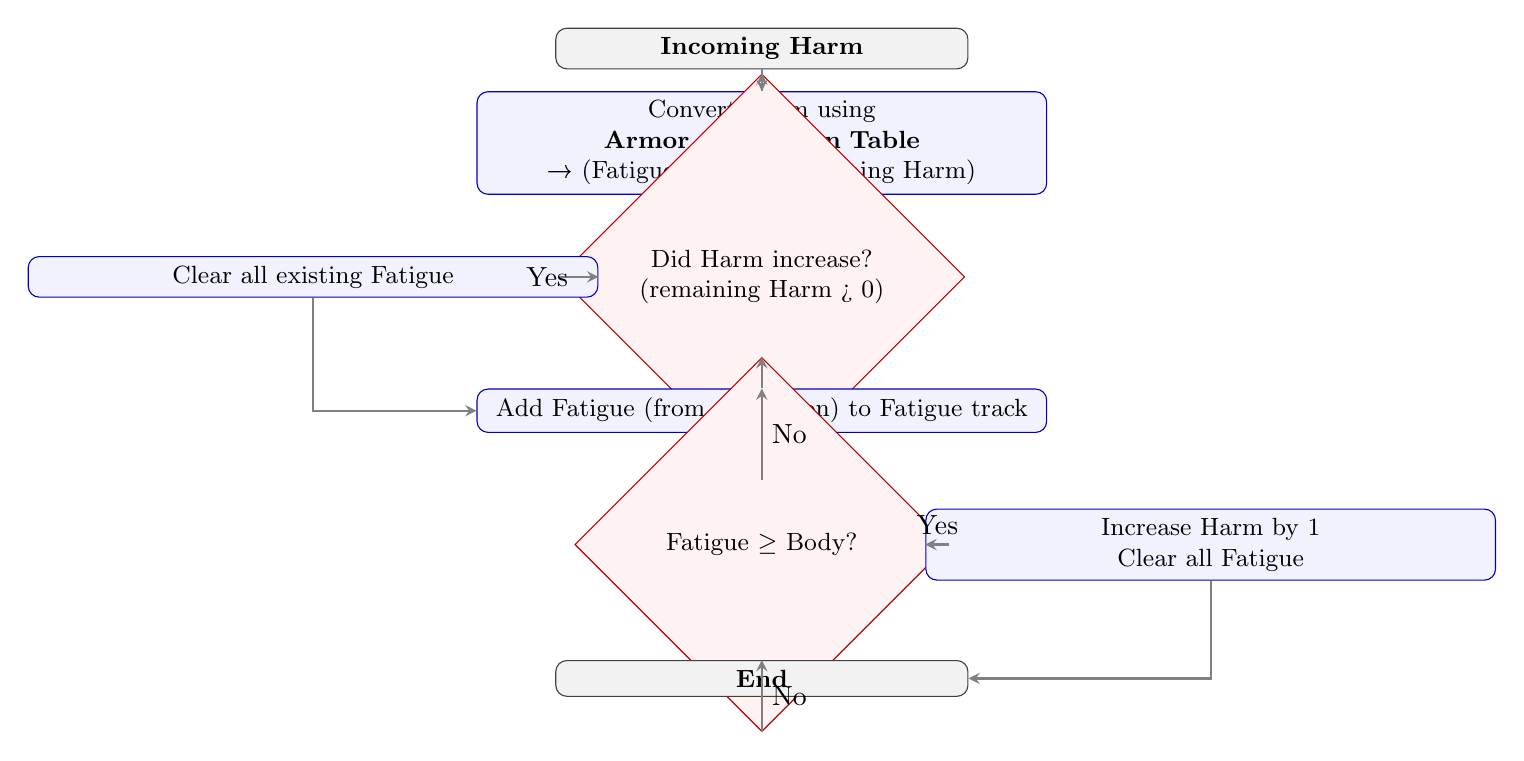
\begin{tikzpicture}[node distance=1.2cm]
\node (start) [startstop] {Incoming Harm};
\node (conv) [process, below of=start] {Convert Harm using\\\textbf{Armor Conversion Table}\\ → (Fatigue amount, remaining Harm)};
\node (dec) [decision, below of=conv, yshift=-0.5cm] {Did Harm increase?\\\small(remaining Harm > 0)};
\node (clear) [process, left of=dec, xshift=-4.5cm] {Clear all existing Fatigue};
\node (addfat) [process, below of=dec, yshift=-0.5cm] {Add Fatigue (from conversion) to Fatigue track};
\node (dec2) [decision, below of=addfat, yshift=-0.5cm] {Fatigue $\geq$ Body?};
\node (overflow) [process, right of=dec2, xshift=4.5cm] {Increase Harm by 1\\Clear all Fatigue};
\node (end) [startstop, below of=dec2, yshift=-0.5cm] {End};

% Arrows
\draw[arrow] (start) -- (conv);
\draw[arrow] (conv) -- (dec);
\draw[arrow] (dec) -- node[anchor=east] {Yes} (clear);
\draw[arrow] (clear) |- (addfat);
\draw[arrow] (dec) -- node[anchor=west] {No} (addfat);
\draw[arrow] (addfat) -- (dec2);
\draw[arrow] (dec2) -- node[anchor=south] {Yes} (overflow);
\draw[arrow] (overflow) |- (end);
\draw[arrow] (dec2) -- node[anchor=west] {No} (end);
\end{tikzpicture}
\end{center}

\vspace{4pt}
\textbf{The “Roller‑Coaster” Effect:}  
When your Harm increases (the armor didn’t soak the whole blow), the shock of the wound clears all your existing Fatigue – you get a second wind just when you’re near collapse. This creates dramatic swings in combat.

\small\textit{Example:} Kael (Body 3, Fatigue 3, Harm 0) takes Harm 1 in Heavy Armor. Conversion → Fatigue 1, remaining Harm 0 → Harm does not increase → Fatigue not cleared. Add Fatigue 1 → Fatigue = 4 (≥ Body 3) → Overflow: Harm 0→1, clear all Fatigue. Final: Harm 1, Fatigue 0.
\end{tcolorbox}

\subsection{Story Beats: The Engine of Drama}
\index{Story Beats (SB)!GM guidance}

Every time a player rolls a 1, you gain Story Beats (SB). These are narrative tools, not punishments.

\begin{tcolorbox}[title=SB Spend Menu, colback=white!97!gray, colframe=black!80!gray]
\begin{tabularx}{\linewidth}{lX}
\toprule
\textbf{SB Cost} & \textbf{Simple Complications} \\
\midrule
1 SB & Minor: noise, distraction, small setback, lost gear, tick a 4/6 clock +1. \\
2 SB & Moderate: alarm raised, new threat enters, lose advantage, worsen Position. \\
3+ SB & Major: reinforcements, scene shifts, stakes escalate, break an asset. \\
\bottomrule
\end{tabularx}
\end{tcolorbox}

\subsection{Failing Forward with SB}
\begin{itemize}
\item \textbf{On Clean Success:} Use SB to add texture. The hero wins, but something changes.
\item \textbf{On Success with SB:} The hero gets what they wanted \emph{and} you spend SB to add further cost or threat.
\item \textbf{On Partial:} Use SB to make the complication sharper.
\item \textbf{On Miss:} Spend SB to escalate the situation.
\end{itemize}

\begin{tcolorbox}[colback=gray!5,colframe=gray!75!black,title=\textbf{Lane Marker: One Complication per Roll}]
When in doubt, spend SB on \emph{one} clear complication instead of many small ones.  
Name it plainly -- "Guard Alerted", "Floor Cracked", "Oath Owed" -- and move on.

Be \textbf{aggressive} with Story Beats, but never arbitrary:
\begin{itemize}[noitemsep]
\item Do not hoard SB -- unused pressure is wasted momentum.
\item Do not invent contrived consequences that ignore the fiction.
\item Spend SB to \emph{sharpen what already matters}, not to add noise.
\end{itemize}
A single, well‑chosen complication should change the situation, not just decorate it.
\end{tcolorbox}

% =========================================================
% OPTIONAL INITIATIVE PROCEDURES
% =========================================================
\section{Optional Initiative Procedures}
\label{sec:optional-initiative}
\index{initiative!optional procedures}

\subsection{Default: Narrative Initiative}
\label{subsec:narrative-initiative-default}
\textbf{By default, Fate's Edge uses narrative initiative.} The GM spotlights characters based on the fiction: the ambushers act first, the character in the most immediate danger reacts, and the pace flows naturally.

\emph{Use the optional structures below only if your table prefers a more structured turn order.} They are fully compatible with the core rules but are not required for balanced play.

\subsection{When to Use Structured Initiative}
Consider structured initiative when:
\begin{itemize}
\item Combat involves six or more participants.
\item Players want a clear, rotating turn order.
\item The table enjoys tactical positioning and resource management.
\item You mix groups with different speeds or reaction times.
\end{itemize}
Even with structured systems, prioritize the fiction: an ambusher still acts first.

\subsection{Option A: Popcorn Initiative}
\label{subsec:popcorn-initiative}
\index{initiative!popcorn}
Each round, the player who just acted chooses who goes next (friend or foe). The GM may veto unrealistic skips (e.g., an archer at Far acting before the enemy in Close).

\begin{table}[h]
\centering
\small
\begin{tabularx}{\linewidth}{lX}
\toprule
\textbf{Step} & \textbf{Procedure} \\
\midrule
1 & Determine first actor by fiction (ambush, fastest PC, etc.). \\
2 & That character takes their full turn. \\
3 & After their turn, they choose any other character who has not acted this round to go next. \\
4 & Repeat until all have acted. \\
5 & End of round: last actor chooses first actor of the next round. \\
\bottomrule
\end{tabularx}
\end{table}

\paragraph{GM Guidance}
Use popcorn initiative to reward clever positioning. Enemies will naturally gang up on vulnerable PCs if players always choose foes -- that's fine. If the table feels unfair, limit choice to "adjacent in fiction" (e.g., only those within Near range).

\subsection{Option B: Side-Based Initiative}
\label{subsec:side-initiative}
\index{initiative!side-based}
All player characters act together, then all enemies act together (or vice versa). Order within the side is negotiated by players.

\begin{table}[h]
\centering
\small
\begin{tabularx}{\linewidth}{lX}
\toprule
\textbf{Step} & \textbf{Procedure} \\
\midrule
1 & Determine which side has surprise or narrative advantage. That side acts first. \\
2 & All members of that side take their turns in any order (players decide). \\
3 & All members of the other side take their turns. \\
4 & Repeat. \\
\bottomrule
\end{tabularx}
\end{table}

\paragraph{GM Guidance}
Best for large combats (10+ combatants). To avoid "alpha strikes," separate enemy groups into two initiatives (e.g., "archers" and "berserkers") that act on different counts.

\subsection{Option C: Speed-Based Slots}
\label{subsec:speed-initiative}
\index{initiative!speed-based}
Each character rolls a die (e.g., 1d10 + Wits) for initiative. Higher scores act first. Ties go to the PC, or roll off.

\begin{table}[h]
\centering
\small
\begin{tabularx}{\linewidth}{lX}
\toprule
\textbf{Step} & \textbf{Procedure} \\
\midrule
1 & At combat start, each player rolls 1d10 + Wits (or other attribute). \\
2 & The GM rolls once for each distinct enemy group (or individually for bosses). \\
3 & Order all participants by score highest to lowest. \\
4 & Act in that order. \\
5 & After each full round, optionally re-roll to reflect changing conditions. \\
\bottomrule
\end{tabularx}
\end{table}

\paragraph{GM Guidance}
Familiar to traditional players. Use a visible tracker (whiteboard, index cards). Re-rolling each round adds chaos but slows play slightly.

\subsection{Mixing Narrative and Structured Initiative}
\label{subsec:mixing-initiative}
Even with a structured system, override it when fiction demands. Examples:
\begin{itemize}
\item A PC triggers a trap mid-round → they act immediately, then initiative resumes.
\item An enemy surrenders → remove them from the order; do not skip a player's turn.
\item A character is delayed (e.g., climbing a wall) → they act at end of round regardless of score.
\end{itemize}
Always state your override clearly: "The bridge collapses---Kaelen, you react first. Everyone else, hold your action."

\subsection{Recommendation for New GMs}
\label{subsec:initiative-recommendation}
Start with \textbf{narrative initiative} for the first 2--3 sessions. Once players are comfortable with Position and DV, introduce \textbf{popcorn initiative} for combat. Reserve side-based or speed-based for large, tactical fights. The best system keeps the fiction moving.

% =========================================================
% PLAYER-MANAGED MODULES
% =========================================================
\section{Standard Rule: Player-Managed Modules}
\label{sec:player-managed-modules-gm}
\index{player-managed modules}\index{GM duties!modules}

This rule makes each player the primary steward of their character-facing trackers (\emph{modules}). It keeps table pace high, reduces hidden bookkeeping, and clarifies when mechanical thresholds trigger. The GM retains authority over world-facing clocks, faction fronts, and major narrative consequences.

\subsection{Scope (What Counts as a Module)}
\label{subsec:module-scope}
Player-managed modules are any \textbf{character-facing} clocks, counters, or discrete states on a single character sheet:
\begin{itemize}
  \item \textbf{Obligation} (per Patron or Symbol)
  \item \textbf{Corruption Clock} (Cantor)
  \item \textbf{Leash} (Summoned spirit strain) and \textbf{Spirit Bond Clock}
  \item \textbf{Repertoire Clock} (Cantor) or similar progression clocks
  \item \textbf{Asset States} (Maintained / Neglected / Compromised / Shattered)
  \item \textbf{Scene Counters} explicitly tied to a PC (Exposure, personal Buff/Debuff durations)
\end{itemize}
\textit{Not included:} GM story resources (global \textbf{Story Beats}), location/faction clocks, and mystery/doom fronts.

\begin{tcolorbox}[colback=black!3,colframe=black!40!white,title={What Players Track (at a Glance)}]
\begin{tabularx}{\linewidth}{lX}
\toprule
\textbf{Module} & \textbf{Owner} & \textbf{Tick / Change Triggers (examples)} \\
\midrule
Obligation (by Patron) & Player & Invoke/Push/ritual text; Invoker \emph{Borrowed Grace}; cracking a Symbol; bargain costs. \\
Corruption Clock & Player & Cantor Push; Resonant Rite; GM spends a Beat tied to the PC's occult actions. \\
Leash (Summoning) & Player & Harm to spirit; commands against nature; split focus; crossing \texttt{[WARD]} (DV = Cap). \\
Spirit Bond [4] & Player & Shared victories, mutual aid, meaningful attempts (once/session/type). \\
Repertoire [6] & Player & Learn a new unique Song/rite-as-song; practice milestones. \\
Asset State (Symbol) & Player & Maintenance/downtime checks; \emph{Crack the Seal} \(\rightarrow\) Compromised; breakage \(\rightarrow\) Shattered. \\
\bottomrule
\end{tabularx}
\end{tcolorbox}

\subsection{Core Principle}
\label{subsec:modules-core}
Players \textbf{immediately} mark their own modules when a rule says "mark +X" or a trigger fires. Threshold effects resolve as soon as reached.

\subsection{Player Duties}
\label{subsec:player-module-duties}
\begin{enumerate}
  \item \textbf{Mark on Cue.} When you Invoke a Rite, Push, spend/clear per rules, or a trigger fires, update your module \emph{now}, not later.
  \item \textbf{Declare Thresholds.} If marking fills a clock or crosses capacity, say so aloud; thresholds resolve before the scene proceeds.
  \item \textbf{State Ownership.} Keep per-Patron Obligation tallies distinct; track each Symbol's state.
  \item \textbf{Keep It Visible.} Use a tracker the GM and table can see (sheet boxes, index cards, or shared digital).
\end{enumerate}

\subsection{GM Duties}
\label{subsec:gm-module-duties}
\begin{enumerate}
  \item \textbf{Spot-Check.} At need, ask any player: current Obligation by Patron, Corruption segments, Leash state, Asset states.
  \item \textbf{Enforce Thresholds.} When a player reports a threshold, apply standard effects \emph{immediately}.
  \item \textbf{Own the Fallout.} Patron intrusions, faction reactions, front clocks, and major narrative consequences remain GM authority.
\end{enumerate}

\subsection{Standard Thresholds \& Effects}
\label{subsec:module-thresholds}
\paragraph{Obligation Capacity}
\label{subsec:obligation-capacity}
\[ \text{Obligation Capacity} = \text{Spirit} + \text{Presence} \]
\begin{itemize}
  \item \textbf{Over Capacity:} Mark \textbf{+1 Fatigue} per segment over capacity.
  \item \textbf{Over \(2\times\) Capacity:} Clear all Fatigue, mark \textbf{+1 Harm (Stress)}, and a \textbf{Patron Intrusion} occurs (GM frames on‑theme demand/complication).
\end{itemize}

\paragraph{Corruption Full}
When a \textbf{Corruption Clock} fills:
\begin{itemize}
  \item Apply the last‑Patron \textbf{benefit \& burden} to the PC (and any listed followers/retainers).
  \item \textbf{Reset} the Corruption Clock to empty.
  \item If the player chooses \textbf{Embrace Corruption}, convert the current Patron theme into a permanent boon/curse (see full rules).
\end{itemize}

\paragraph{Leash Full (Summoning)}
When the \textbf{Leash} fills:
\begin{itemize}
  \item The spirit acts once to its nature, then \textbf{departs} (or turns hostile at GM discretion).
\end{itemize}
\textbf{Leash Capacity:} \(\text{Cap} + \text{Spirit}\) segments. (\textit{Cap} is the outsider's tier: 1 for Lesser, 3 for Greater.)

\paragraph{Symbol State (Invoker)}
\begin{itemize}
  \item \textbf{Maintained} → normal function.
  \item \textbf{Neglected} → GM may impose +1 DV to related rites.
  \item \textbf{Compromised} (e.g., \emph{Crack the Seal}) → instant resolution per rules; mark extra Obligation; repair in Downtime or pay 1 XP.
  \item \textbf{Shattered} → unusable until replaced or ritually restored.
\end{itemize}

\subsection{Table Procedure (90‑Second Loop)}
\label{subsec:module-procedure}
\paragraph{Start of Session}
Players read out: per‑Patron Obligation totals, Corruption segments, standing Asset States, and any personal clocks at 3+.

\paragraph{End of Scene}
Quick pass: "Any marks?" Players tick modules from scene events. If a threshold triggers, resolve now.

\paragraph{Downtime}
Players apply clears (service, contrition, purification, study) to their own modules. GM verifies any costs or fiction.

\subsection{Disputes \& Order of Operations}
\label{subsec:module-disputes}
If two marks land simultaneously, apply them in the \textbf{least advantageous order for the acting character}, unless a rule specifies otherwise. The GM is final arbiter.

\subsection{Accessibility \& Tools}
\label{subsec:module-tools}
Use highly visible trackers: bold boxes on sheets, poker chips for segments, or a shared per‑Patron Obligation table. Keep modules at‑a‑glance to minimize interruption.

\subsection{Worked Micro-Examples}
\label{subsec:module-examples}
\begin{itemize}
  \item \textbf{Invoker Rites Twice:} Vessa Invokes two different Patrons. She marks each Patron's Obligation separately. Hitting capacity with Patron A causes Fatigue; Patron B stays below.
  \item \textbf{Cantor Pushes:} Jorel Pushes a Song (mark +1 Corruption). That fills his clock; he gains last‑Patron boon/burden immediately, then resets to 0.
  \item \textbf{Summoner Clash:} Kestra's Cap~3 elemental takes Harm and crosses a \texttt{[WARD]}; she ticks her Leash twice. On fill, the elemental flares once and departs.
\end{itemize}

% === BEGINNER PATHWAY SIDEBAR ===
\begin{tcolorbox}[title=\textbf{The Core Loop: Your First 10 Games},colback=blue!5,colframe=blue!75!black,fonttitle=\bfseries]
\index{beginner GM advice}
\textbf{Start here for your first session! Ignore advanced systems until comfortable.}

\medskip
1. Player states Goal \& Action (Attribute + Skill)\\
2. GM sets simple DV (2--5)\\
3. Player rolls. Count Successes (6+)\\
4. GM consults Outcome Matrix. \textbf{Ignore Boons for now. Use simple complications on Partial/Miss.}

\medskip
\footnotesize
\textit{Once comfortable, add:} \textbf{Boons} \textbar\ \textbf{Story Beats} \textbar\ \textbf{Clocks}
\end{tcolorbox}

% =========================================================
% FIRST GAME SCENARIO
% =========================================================
\section*{First Game Scenario: The Sunstone Tower}
\addcontentsline{toc}{section}{First Game Scenario: The Sunstone Tower}
\label{sec:sunstone-tower}
\index{first scenario}

\textbf{Premise:} The party is hired to infiltrate the ruined Sunstone Tower and retrieve a magical sunstone before rival treasure hunters do. This scenario uses a limited rules subset perfect for beginners.

\begin{itemize}
\item \textbf{Ignore for this scenario:} Boons, Corruption, intricate magic subsystems, detailed Follower/Asset upkeep.
\item \textbf{Focus on:} Core dice pool, Success/Partial/Miss outcomes, Position, Clocks.
\item \textbf{Character Setup:} Use pregenerated characters or create simple ones with 20 XP and 2--3 clear hooks.
\end{itemize}

\subsection*{GM Prep in 10 Minutes}
\label{subsec:sunstone-prep}
\begin{tcolorbox}[title=Sunstone Tower Prep Checklist, colback=white!97!gray, colframe=black!80!gray]
\begin{itemize}
\item Name 3 NPCs: hirer, rival delver, tower spirit (or echo).
\item Write 1 sentence for each scene: Approach, Interior, Sunstone Chamber.
\item Create 2 clocks: \textbf{Guardian Alert [4]} and \textbf{Tower Collapse [6]}.
\item Decide 1 twist: rival arrives early, tower shifts, or sunstone is not what it seems.
\end{itemize}
\end{tcolorbox}

\subsection*{Scene 1: The Approach}
\label{subsec:sunstone-approach}
\begin{tcolorbox}[colback=gray!5,colframe=gray!75!black,title=\textbf{Lane Marker: Skill Challenge with a Clock}]
\textbf{GM Focus:} Practice calls for DV and Partial outcomes. For this intro, tick the \textbf{Guardian Alert [4]} clock on a Partial or Miss.
\end{tcolorbox}

The tower stands on a cliffside. Players must navigate three challenges:
\begin{itemize}
\item Cross the crumbling bridge (Athletics) -- DV 3
\item Scale the cliff face (Athletics/Strength) -- DV 4  
\item Sneak past the stone guardians (Stealth) -- DV 3
\end{itemize}

\textbf{Guardian Alert Clock [4]:} Each Partial or Miss advances the clock by 1. If filled, guardians activate and pursue; treat them as a single \emph{Tower Guardian} threat with a simple [4] Harm track.

\subsection*{Scene 2: The Tower Interior}
\label{subsec:sunstone-interior}
This scene teaches \textbf{Position} and \textbf{environmental stakes}.

\begin{itemize}
\item \textbf{Dominant:} "You have the high ground on the crumbling staircase, looking down on the patrol."
\item \textbf{Controlled:} "The hallway is dark but quiet. You can take your time, but there might be traps."
\item \textbf{Desperate:} "The floor gives way beneath you as you lunge for the door!"
\end{itemize}

\begin{tcolorbox}[title=How to Set Position in Play, colback=white!97!gray, colframe=black!80!gray]
\index{Position!GM guidance}

\begin{itemize}
\item \textbf{Listen First:} Hear the player's intent and approach. What are they actually doing in the fiction?

\item \textbf{Assess the Situation:} Consider leverage, opposition, time pressure, exposure, and consequences. Ask: \emph{How forgiving is the world right now?}

\item \textbf{Assign the Position:}
\begin{itemize}
  \item \textbf{Dominant}: Clear leverage, surprise, or overwhelming advantage.
  \item \textbf{Controlled}: Stable; mistakes are recoverable.
  \item \textbf{Desperate}: Exposed, rushed, cornered, or facing serious danger.
\end{itemize}

\item \textbf{State It Clearly:} Say it out loud before the roll.  
\emph{"This is Desperate. If it goes wrong, the consequences will be serious."}
\end{itemize}

\textbf{Reminder:} Position is a statement of risk and consequence, not a reward or penalty. It frames what failure \emph{means}.
\end{tcolorbox}

\subsection*{Scene 3: The Sunstone Chamber}
\label{subsec:sunstone-chamber}
The chamber is collapsing as rival delvers close in. Use a simple [6] clock for the collapse. Each round, the clock ticks up by 1. On each Miss, advance it by an extra 1 segment.

\begin{itemize}
\item \textbf{Goal:} Retrieve the sunstone and escape before the clock fills.
\item \textbf{On Fill:} The chamber seals. Escape requires a final, Desperate group action.
\end{itemize}

\begin{tcolorbox}[colback=gray!5,colframe=gray!75!black,title=\textbf{Lane Marker: One New Idea at a Time}]
\footnotesize
Scene 1: Clocks \emph{only}.\\
Scene 2: Add \emph{Position}.\\
Scene 3: Combine \emph{Clocks + Position}. Reserve Boons, Corruption, and advanced magic for later sessions.
\end{tcolorbox}

% =========================================================
% LEARNING THROUGH EXAMPLES
% =========================================================
\section{Learning Through Examples}
\label{sec:learning-examples}
\index{examples!core loop}

This section walks the same situation through multiple passes, adding one rule at a time. Use it as a mental template when you improvise.

\subsection*{Example 1: Core Loop Only}
\label{subsec:ex-core-only}
\begin{tcolorbox}[colback=gray!3,colframe=gray!60,title=\textbf{Example 1 -- No SB, No Boons}]
Lyra tries to sneak past a guardian in a narrow hallway. (Agility + Stealth = 5d10).\\
GM: normal risk, DV 3, Controlled Position.\\
Roll: 3, 5, 6, 7, 9 → 3 successes (6,7,9).\\[0.3em]
DV 3 with 3 successes = \textbf{Success}.\\[0.3em]
GM: "You slip past the guardian quietly. You're in position behind it if you want to act."
\end{tcolorbox}

\subsection*{Example 2: Add Story Beats Only}
\label{subsec:ex-sb-only}
\begin{tcolorbox}[colback=gray!3,colframe=gray!60,title=\textbf{Example 2 -- Adding Story Beats}]
Same situation. Lyra rolls 5d10: 1, 4, 6, 6, 8.\\
Successes: 3 (6,6,8). One 1 → 1 SB for GM.\\[0.3em]
DV 3 with 3 successes = \textbf{Success} with 1 SB.\\[0.3em]
GM spend (1 SB = Minor): "You get past the guardian, but your cloak snags and tears. The sound echoes -- the next room has a -1 Position penalty for stealth checks."
\end{tcolorbox}

\subsection*{Example 3: Add Boons Only}
\label{subsec:ex-boons-only}
\begin{tcolorbox}[colback=gray!3,colframe=gray!60,title=\textbf{Example 3 -- Adding Boons}]
Later, Lyra scales a loose stone wall (Athletics + Agility = 4d10). DV 3.\\
Roll: 2,3,4,5 → 0 successes = \textbf{Miss}.\\[0.3em]
GM awards \textbf{2 Boons}. "You slip and land hard, taking 1 Harm. Mark 2 Boons -- you can use them later to turn the tide."\\
Next attempt, Lyra spends 1 Boon to re-roll a die, turning failure into success.
\end{tcolorbox}

\subsection*{Example 4: Putting It Together}
\label{subsec:ex-full}
\begin{tcolorbox}[colback=gray!3,colframe=gray!60,title=\textbf{Example 4 -- SB + Boons + Position}]
The party flees as the tower collapses. A crumbling staircase blocks the exit.\\
GM: "Desperate. DV 4 to get everyone across safely."\\
Lyra leads, rolling 6d10 (Agility + Athletics + help): 1,2,6,7,7,9.\\
4 successes vs DV 4 = Success. 1 rolled 1 = 1 SB to GM. Desperate Position.\\
GM: "You all make it across, but the last step collapses behind you. I spend 1 SB: your exit path is gone. You'll need a new way out."\\
\textbf{Lesson:} Even on a success, SB let you bend the fiction toward drama without erasing the player's win.
\end{tcolorbox}

% =========================================================
% COMBAT SIMPLIFIED
% =========================================================
\section{Combat Made Simple}
\label{sec:combat-simple}
\index{combat!simplified}

Combat uses the same core loop. The stakes are higher and more immediate.

\begin{tcolorbox}[title=Combat Quick Reference, colback=white!97!gray, colframe=black!80!gray]
\index{combat!quick reference}
\begin{itemize}
\item \textbf{Initiative:} No fixed order. Ask: "Who acts next?" Follow the fiction.
\item \textbf{Actions:} Each turn, a character can move and take one meaningful action.
\item \textbf{Position Matters:} Flanking or ambush → Dominant; surrounded or exposed → Desperate.
\item \textbf{Use Clocks:} Track enemy morale [6], environmental dangers [4], and boss thresholds.
\end{itemize}
\end{tcolorbox}

\subsection{Three-Beat Combat Structure}
\label{subsec:three-beat-combat}
When lost in a fight, fall back on three beats:
\begin{enumerate}
\item \textbf{Opening Exchange:} Establish where everyone is and what they want.
\item \textbf{Turning Point:} Spend SB or tick clocks to change the situation (reinforcements, terrain shifts).
\item \textbf{Final Gamble:} Make the last few rolls matter -- higher DV, Desperate Position, or big rewards.
\end{enumerate}

\begin{tcolorbox}[colback=gray!5,colframe=gray!75!black,title=\textbf{Example: SB in Combat}]
The party fights bandits on a collapsing bridge.\\
On a Partial, GM spends 2 SB: "You push them back, but the bridge loses another support. The \emph{Bridge Collapse [4]} clock advances."\\
Now every action is also about whether they escape in time.
\end{tcolorbox}

% =========================================================
% CLOCKS & FRONTS
% =========================================================
\section{Clocks \& Fronts}
\label{sec:clocks-fronts}
\index{clocks!GM guidance}\index{fronts}

Clocks are visual trackers for threats, progress, and looming changes. They keep pressure visible and shared.

\subsection{Basic Clock Usage}
\label{subsec:clock-usage}
\begin{itemize}
\item \textbf{Size:} [4] for small scenes, [6] for bigger problems, [8] for arcs.
\item \textbf{Advance On:} Misses, certain Partials, or SB spends.
\item \textbf{Name It:} "Alarm Raised [4]" or "Floodwaters Rise [6]" is better than a blank circle.
\end{itemize}

\begin{tcolorbox}[title=Beginner Clock Limits, colback=white!97!gray, colframe=black!80!gray]
\begin{itemize}
\item No more than 3 active clocks per scene.
\item Only 1--2 clocks should matter to the current roll.
\item Say out loud when you tick a clock and why.
\end{itemize}
\end{tcolorbox}

\subsection{Mini-Fronts for Short Arcs}
\label{subsec:mini-fronts}
A \emph{Front} is a cluster of related clocks and threats.
\begin{itemize}
\item \textbf{Example Front:} "Rival Delvers of the Sunstone Tower"
\item Clocks: "Rivals Close In [6]", "Tower Integrity [6]", "Rival Reputation [4]".
\item Each time you spend SB, consider ticking one of these clocks.
\end{itemize}

% =========================================================
% MODULAR PATHWAYS
% =========================================================
\section{Ready for More? Add These Systems}
\label{sec:modular-systems}
\index{optional systems}

Once comfortable with the core loop, introduce these modules one at a time. Treat each as a new lane marker.

\subsection{Boons}
\label{subsec:boons-gm}
Boons reward players for pushing their luck.
\begin{itemize}
\item On \textbf{Miss:} Gain 2 Boons.
\item On \textbf{Partial:} Gain 1 Boon.
\item \textbf{Spend:} Re-roll a die, add +1 Effect, or seize a small advantage (GM‑approved).
\end{itemize}
Start with \emph{re-roll only}. Once players are comfortable, add the other options.

\subsection{Advanced Magic}
\label{subsec:advanced-magic}
\begin{itemize}
\item \textbf{Basic:} Use simple Tag-based magic (single roll, single tag).
\item \textbf{Intermediate:} Add Runekeepers after 2--3 sessions, when everyone understands SB and Clocks.
\item \textbf{Advanced:} Introduce Invokers and ritual magic for groups that enjoy planning and complex payoffs.
\end{itemize}

\subsection{Followers, Assets, and Domains}
\label{subsec:followers-assets}
Add persistent resources when the group cares about territory, organizations, or long‑term projects.
\begin{itemize}
\item Start with 1 simple Follower or Asset each.
\item Tie them to clocks: "Caravan Reputation [6]", "Temple Influence [4]".
\item Spend SB to threaten or complicate these resources.
\end{itemize}

% =========================================================
% ABSTRACTION
% =========================================================
\section{Abstracting Time and Currency}
\label{sec:abstraction}
\index{time!narrative abstraction}\index{currency!abstraction}

Fate's Edge uses \textbf{narrative time} and \textbf{abstract wealth} to keep the focus on story, not bookkeeping.

\subsection{Narrative Time (Not Minutes)}
\label{subsec:narrative-time}
Describe durations in narrative beats, not concrete minutes or hours. Use these units:

\begin{center}
\small
\begin{tabular}{ll}
\toprule
\textbf{Narrative Unit} & \textbf{When to Use} \\
\midrule
A moment & One action, a heartbeat, a single exchange \\
Some time & A few minutes -- picking a lock, searching a room \\
Significant time & Hours -- a ritual, a short rest, a negotiation \\
Half a day & Morning to noon, dusk to midnight \\
A day & Dawn to dusk, including travel or major activity \\
\bottomrule
\end{tabular}
\end{center}

\paragraph{Example:}
Instead of "It takes 20 minutes to climb the tower", say: "It takes \textbf{significant time} -- long enough for the patrol to pass and return." That keeps pressure without a stopwatch.

\subsection{Abstract Currency (XP as Coin)}
\label{subsec:xp-as-coin}
Fate's Edge abstracts most coinage and barter. Exceptional expenses, bribes, or lifestyle costs are handled through \textbf{Boons}, \textbf{Assets}, or \textbf{Story Beats} -- not copper counting.

When a player needs to pay for something significant and has no relevant Asset or favor, they may spend \textbf{XP}. Treat 1 XP as a substantial bribe, emergency fund, or major purchase.

\begin{tcolorbox}[title=When to Use XP for Coin, colback=white!97!gray, colframe=black!80!gray]
\index{XP!as currency}
\textbf{Appropriate uses:}
\begin{itemize}
\item Bribing a corrupt official (2--4 XP)
\item Outfitting a small expedition (1 XP per full kit)
\item Buying a rare magical component (2--3 XP)
\item Establishing a modest safehouse (4 XP, counts as Minor Asset)
\end{itemize}
\textbf{Inappropriate uses:}
\begin{itemize}
\item Routine meals, lodging, or travel supplies (cover with narrative)
\item Anything that would trivialize a previous asset purchase
\item Repeated, low‑stakes expenses
\end{itemize}
\end{tcolorbox}

\paragraph{GM Guidance:}
Spending XP for coin should feel like a meaningful sacrifice, not a tax. Always ask: "Is this advancing the story?" If yes, allow it. If not, offer a different cost (a Boon, a Debt, a Story Beat). This keeps material concerns from derailing the narrative.

% =========================================================
% SESSION FLOW
% =========================================================
\section{Session Flow: A GM Cognitive Checklist}
\label{sec:session-flow}
\index{session flow!checklist}

Use this as a quiet mental script. You do not need to say any of it out loud.

\subsection{Opening 10 Minutes}
\label{subsec:opening-10}
\begin{itemize}
\item Ask: "What does everyone want out of tonight?" (goal, vibe, focus).
\item Recap 2--3 key facts and 1 unresolved clock.
\item Ask each player: "What is your character worried about right now?"
\end{itemize}

\subsection{During Play}
\label{subsec:during-play}
\begin{itemize}
\item Before a roll: Name DV, Position, and stakes.
\item After a roll: Say the outcome type (Clean Success/Success with SB/Partial/Miss) first, then the fiction.
\item Between scenes: Look at clocks. Ask, "Which one should move? What changes in the world?"
\end{itemize}

\subsection{Closing 10 Minutes}
\label{subsec:closing-10}
\begin{itemize}
\item Ask: "What was your favorite moment?" (signals what to do more of).
\item Note any clocks that reached halfway or full.
\item Jot 2 bullet points: "Next time on Fate's Edge..." as hooks.
\end{itemize}

\begin{tcolorbox}[title=\textbf{Quick GM Cheat Sheet},colback=green!5,colframe=green!75!black]
\index{GM cheat sheet}
\begin{itemize}
\item \textbf{DV Default:} 3 (adjust ±1 for ease/difficulty).
\item \textbf{Position:} Controlled (normal), Dominant (advantage), Desperate (risk).
\item \textbf{SB Spend:} 1=minor, 2=moderate, 3+=major complication.
\item \textbf{Max Clocks:} 3 per scene to avoid overwhelm.
\item \textbf{Golden Rule:} When in doubt, make a ruling that keeps the story moving.
\end{itemize}
\end{tcolorbox}

\vspace{1em}
\noindent\textbf{Remember:} The goal is to tell an exciting story together. These rules are tools, not tests. Start simple, add complexity when ready, and keep lane markers clear: one new idea at a time, one clear consequence per roll, and one or two clocks that really matter.

\clearpage
\begin{tcolorbox}[colback=blue!5!white, colframe=blue!75!black, boxrule=0.5pt, arc=2mm, left=6pt, right=6pt, top=6pt, bottom=6pt]
\begin{center}
\textbf{\large The GM Mindset: Three Guiding Principles}
\end{center}
\medskip
\small
\begin{tabularx}{\linewidth}{>{\bfseries}p{0.25\linewidth} X}
\toprule
Principle & Guidance \\
\midrule
1. Don't Fear Failure &
The dice are not your opposition---they are your collaborators.  
When unsure, ask: \emph{"Does this create a more interesting story?"}  
If yes, lean into it. The system rewards bold GM decisions with momentum, not penalties. \\
\addlinespace
2. Spend SB to Create &
Every Story Beat should open a new door, not close one.  
"The door slams shut" is weaker than "the door slams shut -- but the echo draws guards closer."  
Favor movement, pressure, and consequences over hard stops. \\
\addlinespace
3. The Real DV Is in Stakes &
If a scene feels flat, raise the stakes -- not the difficulty.  
Before the roll, be clear about what failure means.  
When players ask "What happens if I fail?", answer honestly.  
That answer is where tension lives, not in higher numbers. \\
\bottomrule
\end{tabularx}
\end{tcolorbox}

\clearpage
\begin{tcolorbox}[colback=black!3!white,colframe=black!40!white,title={Encounter in Action: The Ambush at Raven's Ford}]
\label{box:ambush-example}
\index{example!combat encounter}
This example shows how the core systems---narrative initiative, Story Beats, Boons, Bonds, and damage---come together in play. The party consists of \textbf{Thane} (fighter), \textbf{Sariel} (rogue), and \textbf{Kestra} (mage).

\subsection*{Setup}
The group crosses a rope bridge when two bandits attack from the far side. GM sets the scene:
\begin{quote}
"The bridge sways under your feet. Two crossbowmen take aim from behind a boulder. Thane, you're closest to them. Sariel is mid‑bridge, Kestra still on the near cliff."
\end{quote}
No initiative rolled. GM asks: "Who acts first?" Thane says, "I charge." The GM agrees -- he's closest and has momentum.

\subsection*{Round 1 --- Thane's Turn}
Thane rushes the bandits. GM: "Exposed on the bridge, crossbows trained on you -- Desperate, DV 3 to reach them before they shoot." Thane rolls Body + Melee (6d10): 7,5,4,2,1,1 → two successes (7 only). One short → Miss.

\paragraph{Result:} GM gains 2 SB (two 1s) and player gains 2 Boons. GM narrates:
\begin{quote}
"You make it halfway, but a bolt grazes your arm. Mark Harm 1. The bandits draw swords -- they're in Close now."
\end{quote}

\subsection*{Enemy Turn (No Roll)}
Because Thane closed the distance, bandits "draw swords" as a consequence of his Miss. GM uses the 2 SB:
\begin{itemize}
  \item \textbf{Spend 1 SB:} "The second bandit kicks a loose plank. The bridge lurches -- everyone make Body + Athletics (DV 3) or be knocked Prone."
  \item \textbf{Spend 1 SB:} "Sariel, your footing slips; your next action is Desperate."
\end{itemize}
Sariel fails; she is Prone. Kestra succeeds.

\subsection*{Player Turn --- Sariel Uses a Boon}
Sariel stabs the nearest bandit from prone. GM: "Desperate, DV 3." She rolls: no successes → Miss, gains 2 Boons (now has 2 total). Before GM narrates failure, she \textbf{spends 1 Boon} to re-roll one die. Re-roll comes up 6 → adds one success, turning Miss into Partial. GM: "You slash his leg -- he drops to one knee, but your dagger is lodged. It'll take a moment to free it."

\subsection*{Bond Transfer}
Kestra has a Bond with Sariel ("She saved me once; I owe her"). As a free action (Tier III+), Kestra \textbf{transfers 2 Boons} to Sariel. Sariel now has 3 Boons.

\subsection*{Kestra's Turn --- Boon for Environmental Effect}
Kestra uses magic to collapse part of the bridge behind the bandits. She has \textbf{Spellcraft} and \texttt{[EARTH]}, \texttt{[BREAK]}. GM: "Controlled, DV 4. Spend a Boon to improve to Dominant?" Kestra spends 1 Boon (now Dominant, DV 4). She rolls successfully, generating 1 SB (a 1). GM spends that SB immediately:
\begin{quote}
"The bridge splinters -- the bandits are isolated! But the shockwave also loosens the rope on your side. New Clock: Bridge Collapse [4]."
\end{quote}
Damage not rolled. Bandits stranded -- a fictional consequence.

\subsection*{End of Encounter}
Sariel, with extra Boons, frees the dagger and finishes the wounded bandit (Clean Success). The other bandit surrenders. No enemy "damage" rolled; all consequences came from SB, Position, and player choices.

\paragraph{Key Takeaways}
\begin{itemize}
\item Initiative is narrative -- whoever makes sense acts first.
\item Enemies do not roll to hit. Their actions are consequences of PC misses or SB spends.
\item Boons can re‑roll, shift Position, create environmental effects, or be shared via Bonds.
\item Damage (Harm) is applied directly from fiction, not from an enemy "attack roll."
\end{itemize}
\end{tcolorbox}

% =========================================================
% THRESHOLD EFFECTS (FIXED: No longtable, using tabularx in box)
% =========================================================
\section{Threshold Effects Reference}
\label{sec:threshold-effects}
\index{thresholds!effects table}

When a player announces \textbf{"I cross the threshold"} -- a doorway, a riverbank, a crossroads, the space between sleeping and waking -- use this table to determine the immediate effect. Thresholds are where the world's memory is thinnest; crossing them without respect invites attention.

\begin{tcolorbox}[
  colback=blue!5!white,
  colframe=blue!75!black,
  title=GM Procedure for Threshold Crossings,
  fonttitle=\bfseries
]
\begin{enumerate}
  \item Ask the player to describe \textbf{how} they cross (e.g., "I step over the river stone," "I open the door with my left hand").
  \item Based on their description, set \textbf{Position} (Dominant/Controlled/Desperate).
  \item Apply the effect from the table below. If the player showed respect (offering, announced name, proper etiquette), improve Position by one step.
  \item Optionally, spend SB to escalate (see \texttt{SB Spend Opportunity} column).
\end{enumerate}
\end{tcolorbox}

\medskip
\begin{tcolorbox}[
  colback=white!97!gray,
  colframe=black!80!gray,
  title=Threshold Effects Table,
  fonttitle=\bfseries
]
\small
\begin{tabularx}{\linewidth}{p{2.2cm}p{2.8cm}p{2.2cm}p{2.8cm}}
\toprule
\textbf{Threshold Type} & \textbf{Typical Effect} & \textbf{SB Spend Opportunity} & \textbf{Respectful Crossing} \\
\midrule
Doorway (unwarded) & Position worsens one step (attention from spirits). & 1 SB: door leads to wrong room. & Knock first; announce your name. \\
Doorway (warded) & Resolve test (DV 3) or mark 1 Fatigue. & 2 SB: ward triggers (Harm 1). & Offer a coin or a hair. \\
Crossroads & GM asks a "choice" question; answer becomes true for the scene. & 3 SB: a stranger appears with a bargain. & Leave a stone at the centre. \\
Riverbank & Roll Spirit + Survival (DV 3); success gives a vague omen. & 2 SB: spirit from the water surfaces. & Pour a libation before drinking. \\
Bridge & Player must state a memory aloud; the bridge "remembers" it. & 3 SB: bridge demands a toll (1 Fatigue). & Walk at the centre; do not run. \\
Sleep/waking edge & Player narrates a dream fragment; GM gains 1 SB. & 4 SB: dream becomes real for one exchange. & Sleep with a red thread on the wrist. \\
Forest path & Navigate test (DV 3) or lose 1 segment of travel progress. & 2 SB: trees shift; path loops back. & Tie a thread to a branch before entering. \\
Threshold of a home & First social roll inside gains +1 Position (guest‑right). & 1 SB: a portrait watches you. & Remove your shoes; wait to be invited. \\
Graveyard gate & Spirit + Resolve (DV 3) or feel a cold hand on your shoulder. & 3 SB: an Echo manifests and asks a question. & Leave a coin on the nearest grave. \\
\bottomrule
\end{tabularx}
\end{tcolorbox}

\subsection*{Threshold Clocks}
\index{clocks!threshold instability}
For a location that is heavily liminal (a haunted manor, a fey crossing, a dungeon built on a ley line), start a \textbf{Threshold Instability [4--6]} clock. Tick it each time a player crosses a threshold without proper respect (no offering, no announced name, no etiquette). When the clock fills:

\begin{itemize}
  \item Doors open to the wrong rooms.
  \item The dead walk for one scene.
  \item The party is lost in a mirror realm and must find their way out (treat as a Travel Clock [6]).
\end{itemize}

\subsection*{Player‑Driven Thresholds}
When a player says "I act at the threshold," encourage them to be specific. The GM uses that fiction to set Position:

\begin{itemize}
  \item \textbf{Respectful crossing} (removing boots, pouring a libation, speaking a name) → Position starts one step higher (e.g., Controlled → Dominant).
  \item \textbf{Brazen crossing} (kicking the door open, stepping over without acknowledgment) → Position starts one step lower (e.g., Controlled → Desperate).
\end{itemize}

\subsection*{Example}
The party stands before a moss‑covered door in the Mistlands.  
\textbf{Player:} "I knock three times, then say 'guest seeking shelter'."  
\textbf{GM (respectful crossing):} "Dominant Position. Roll Spirit + Sway (DV 2) to see if the house welcomes you."  

If the player had kicked the door, the GM would set Desperate Position and tick the \emph{Threshold Instability} clock.
